16. 如图,正方形ABCD是表示某地区的近似图,若已知M、N为线段BD的三等分点,点E是线段BC的三等分点,三角形MEN为该区域内的一块沙漠,求:(1)该地区的土地沙漠化率是多少?(除不尽的百分号前保留一位小数)(2)据科学家测算,该地区若再不采取措施,则10年后,三角形BEM 地区也会被沙漠化,请计算10年后该地区的沙漠面积比10年前增加了百分之几?

\begin{flushright}

    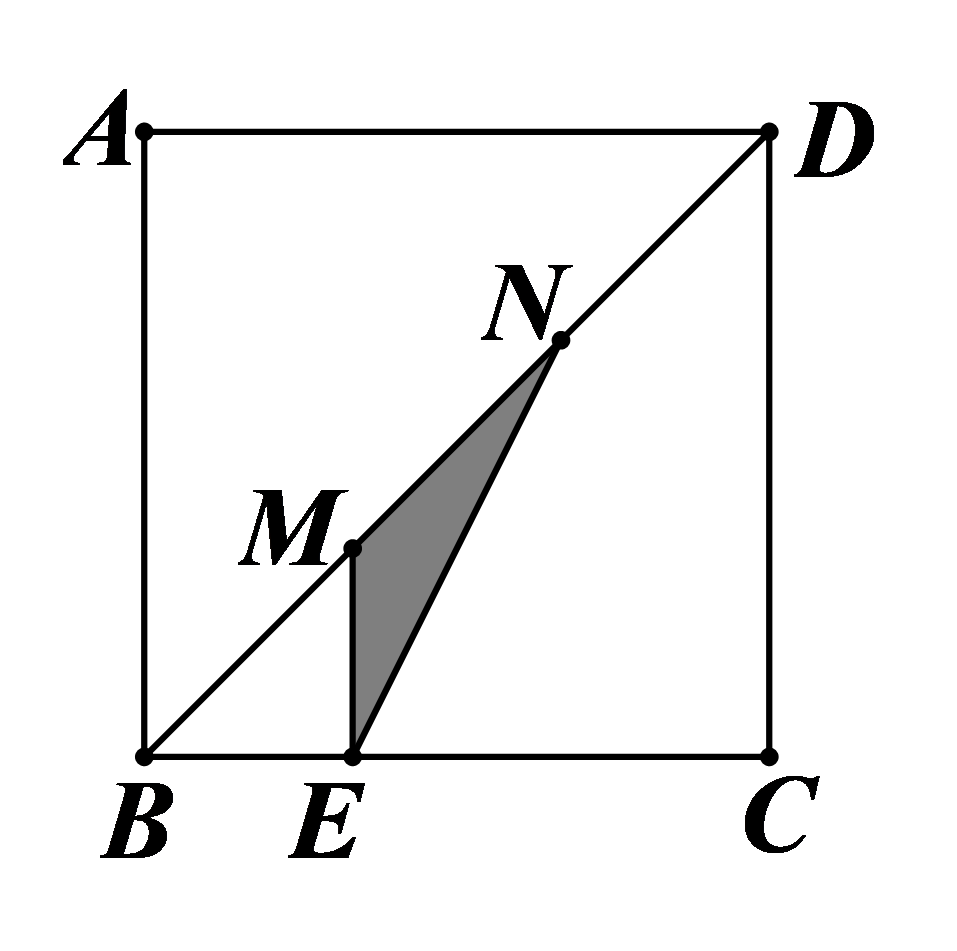
\includegraphics[height=3cm]{lib/image/MJA03050116.png}

\end{flushright}



